\section{Surface covering}
\label{sec:9}

\begin{figure*}[b]
    \centering
    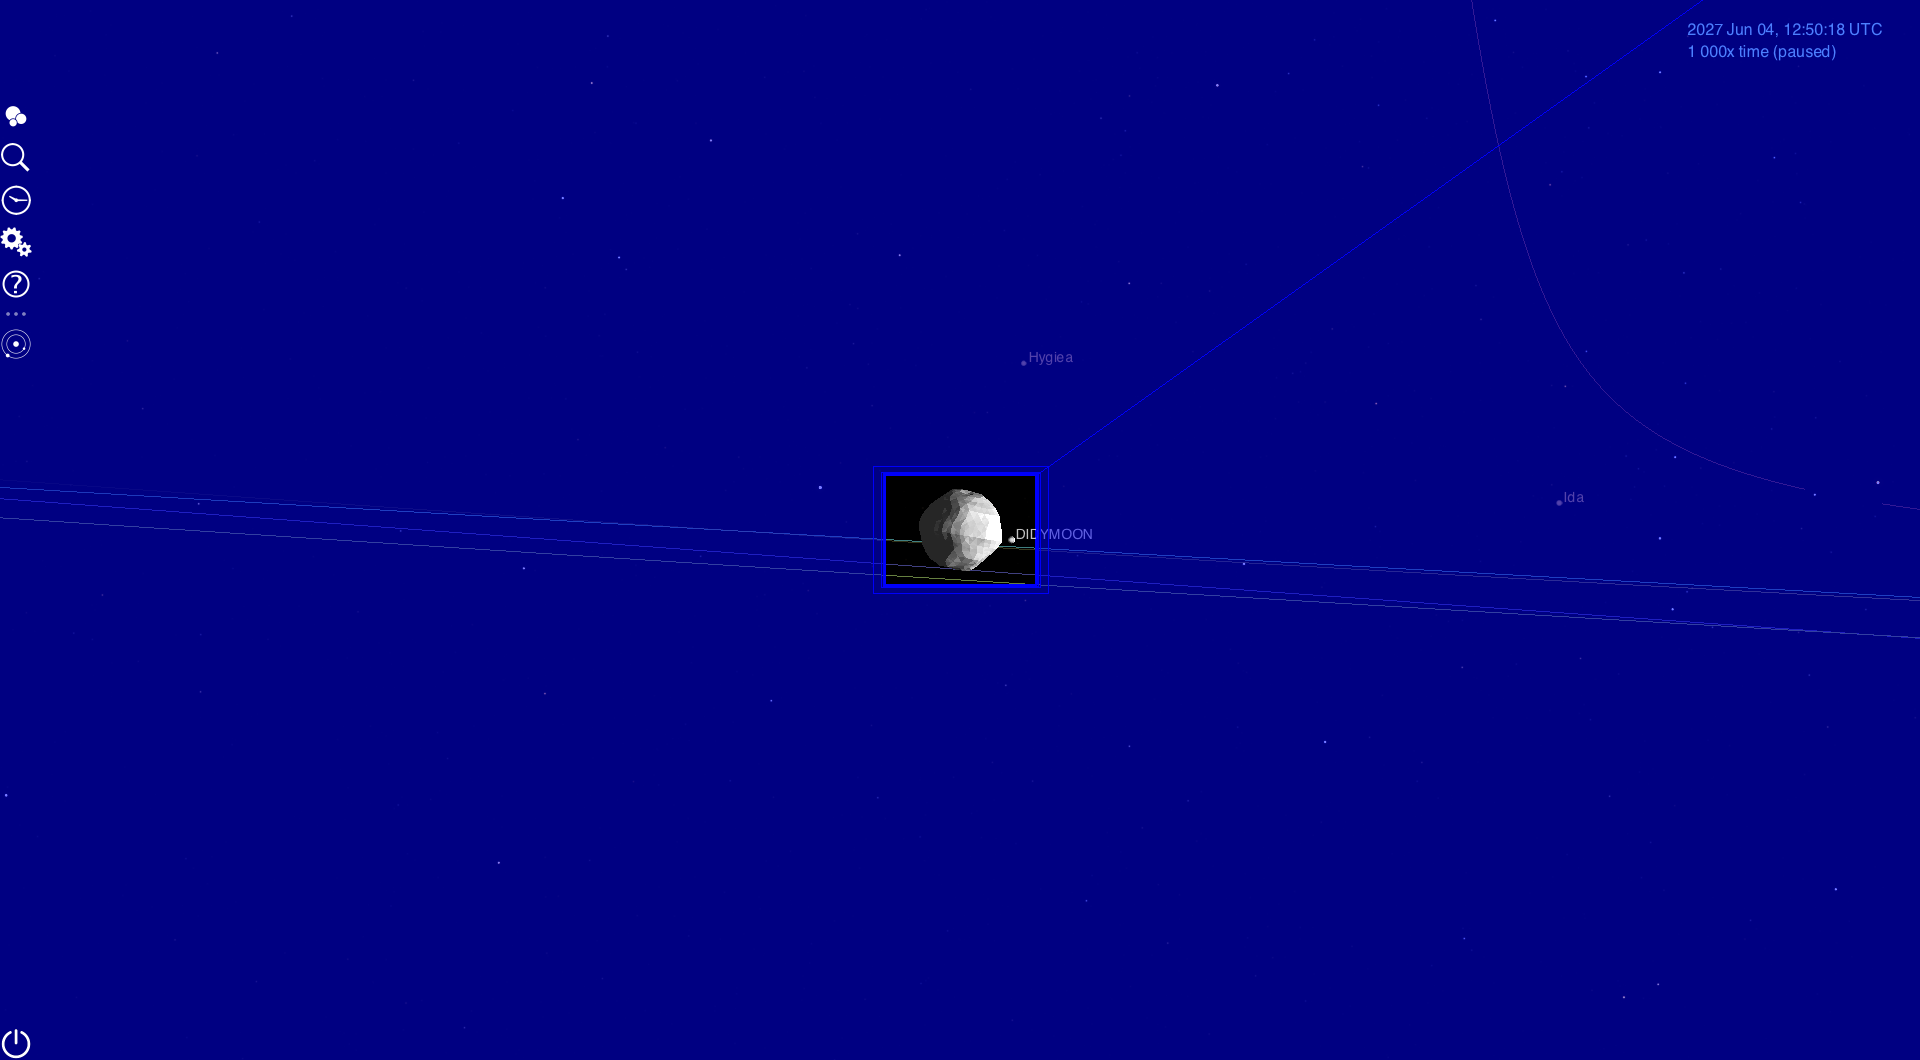
\includegraphics[width=0.45\linewidth]{rsc/cosmo1.png}
    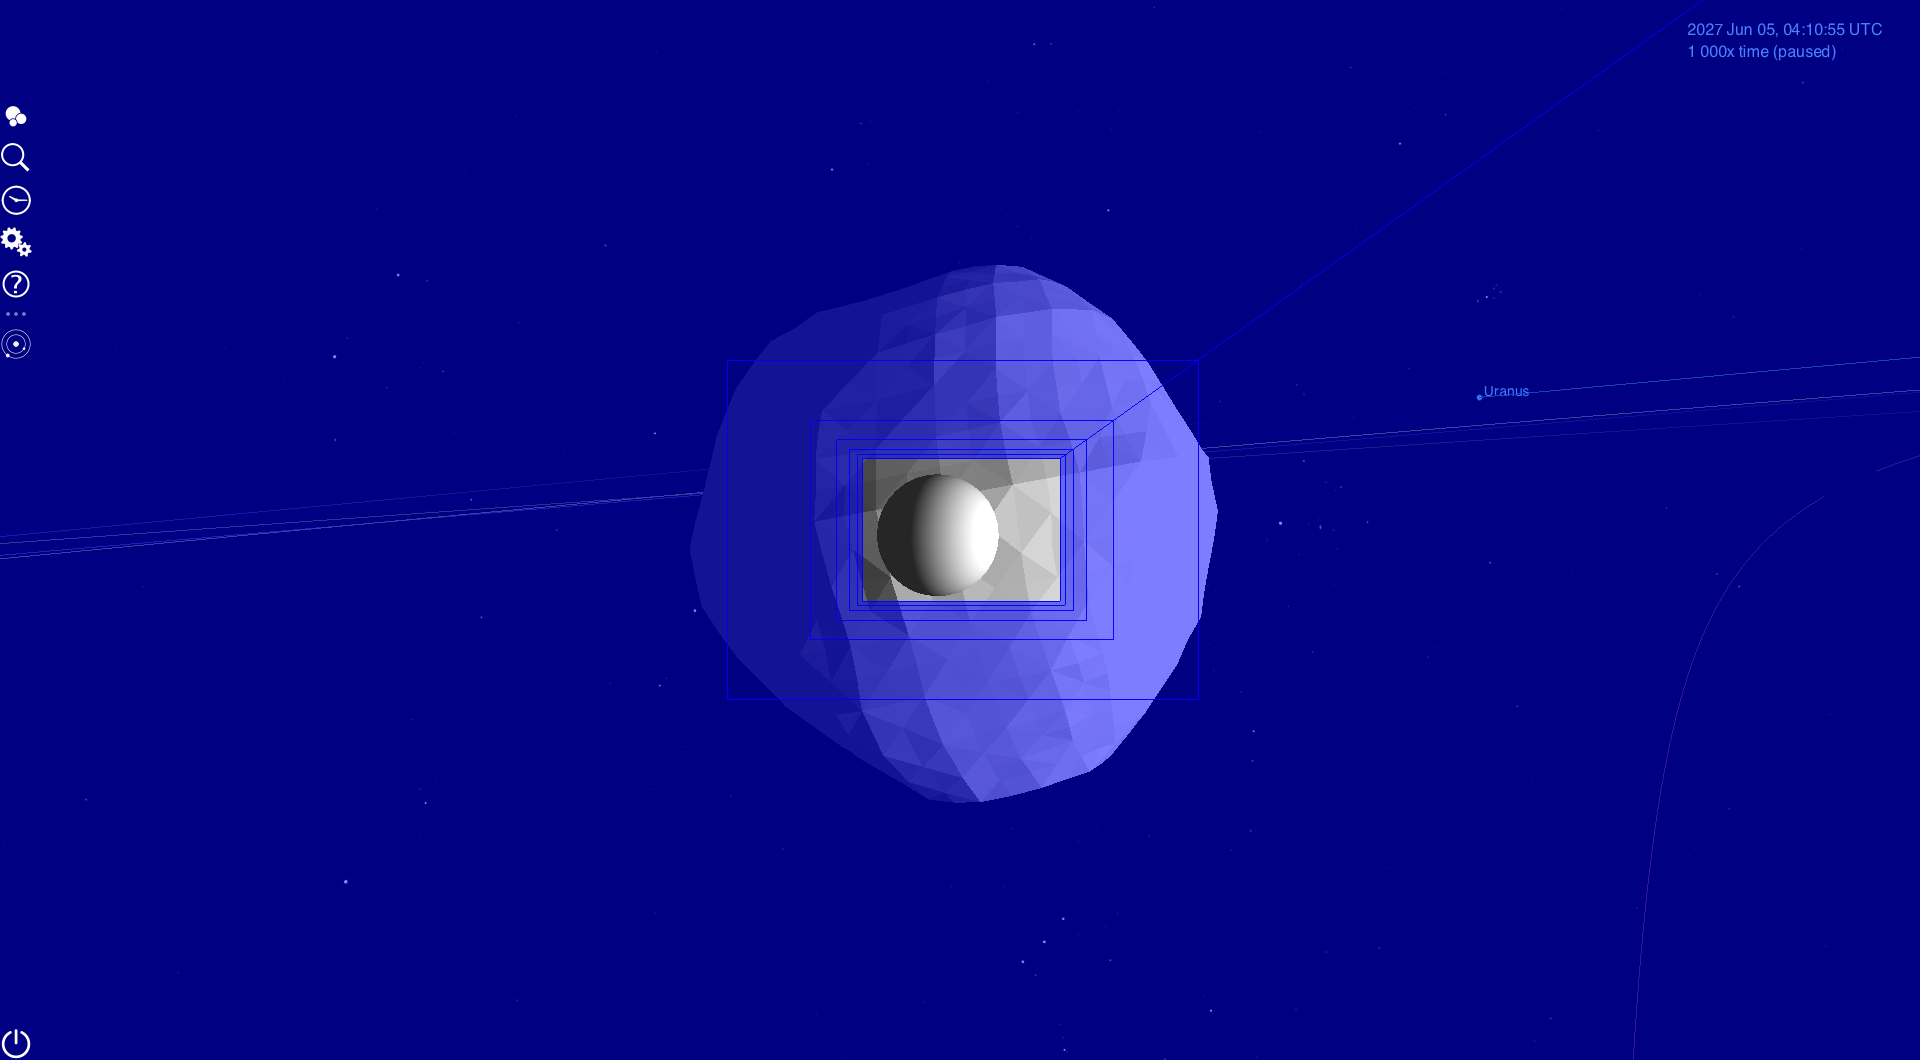
\includegraphics[width=0.45\linewidth]{rsc/cosmo2.png}
    \caption{View from HERA on the binary system of asteroids Didymos from Cosmographia. The field of view of the camera imaging appears in blue. The first image is the previous rotation before the closest flyby on June 24, 2024, at 12:50, and the second image is during the closest flyby of 1 \si{AU} on June 25, 2024, at 4:00.}
    \label{fig:9.1}
\end{figure*}

\begin{figure*}[t]
    \centering
    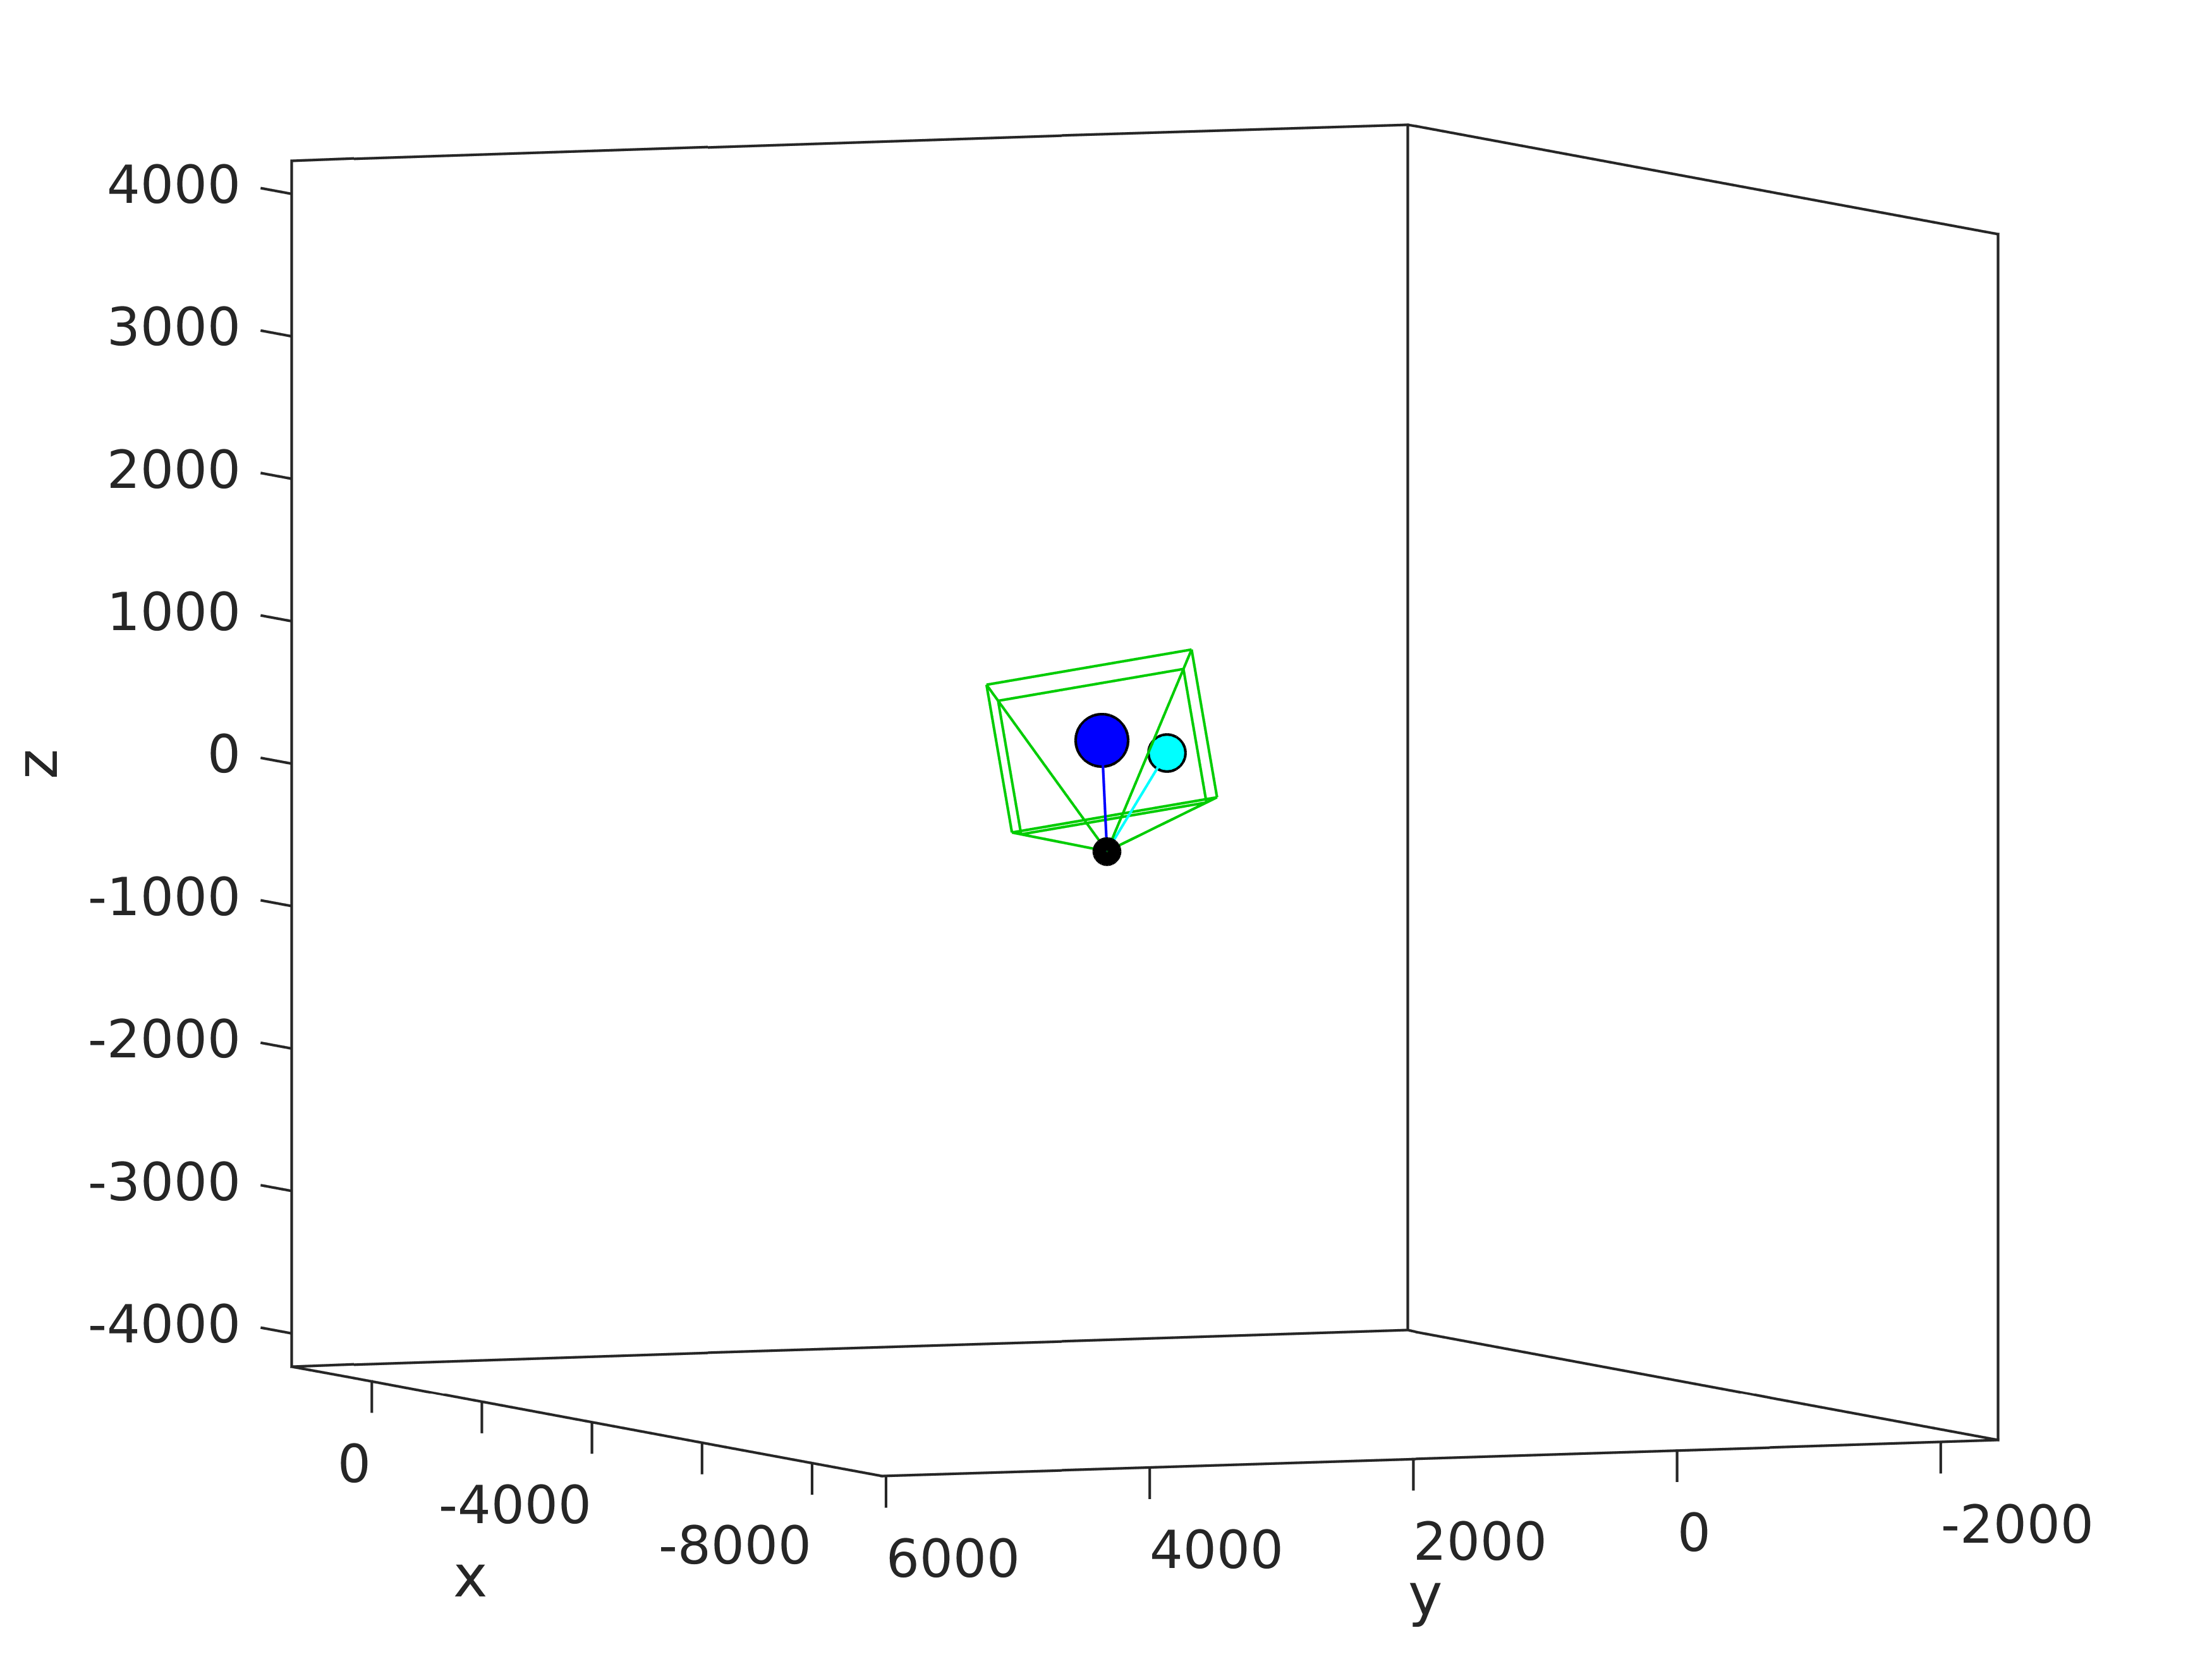
\includegraphics[width=0.49\linewidth]{rsc/cosmo-matlab1.png}
    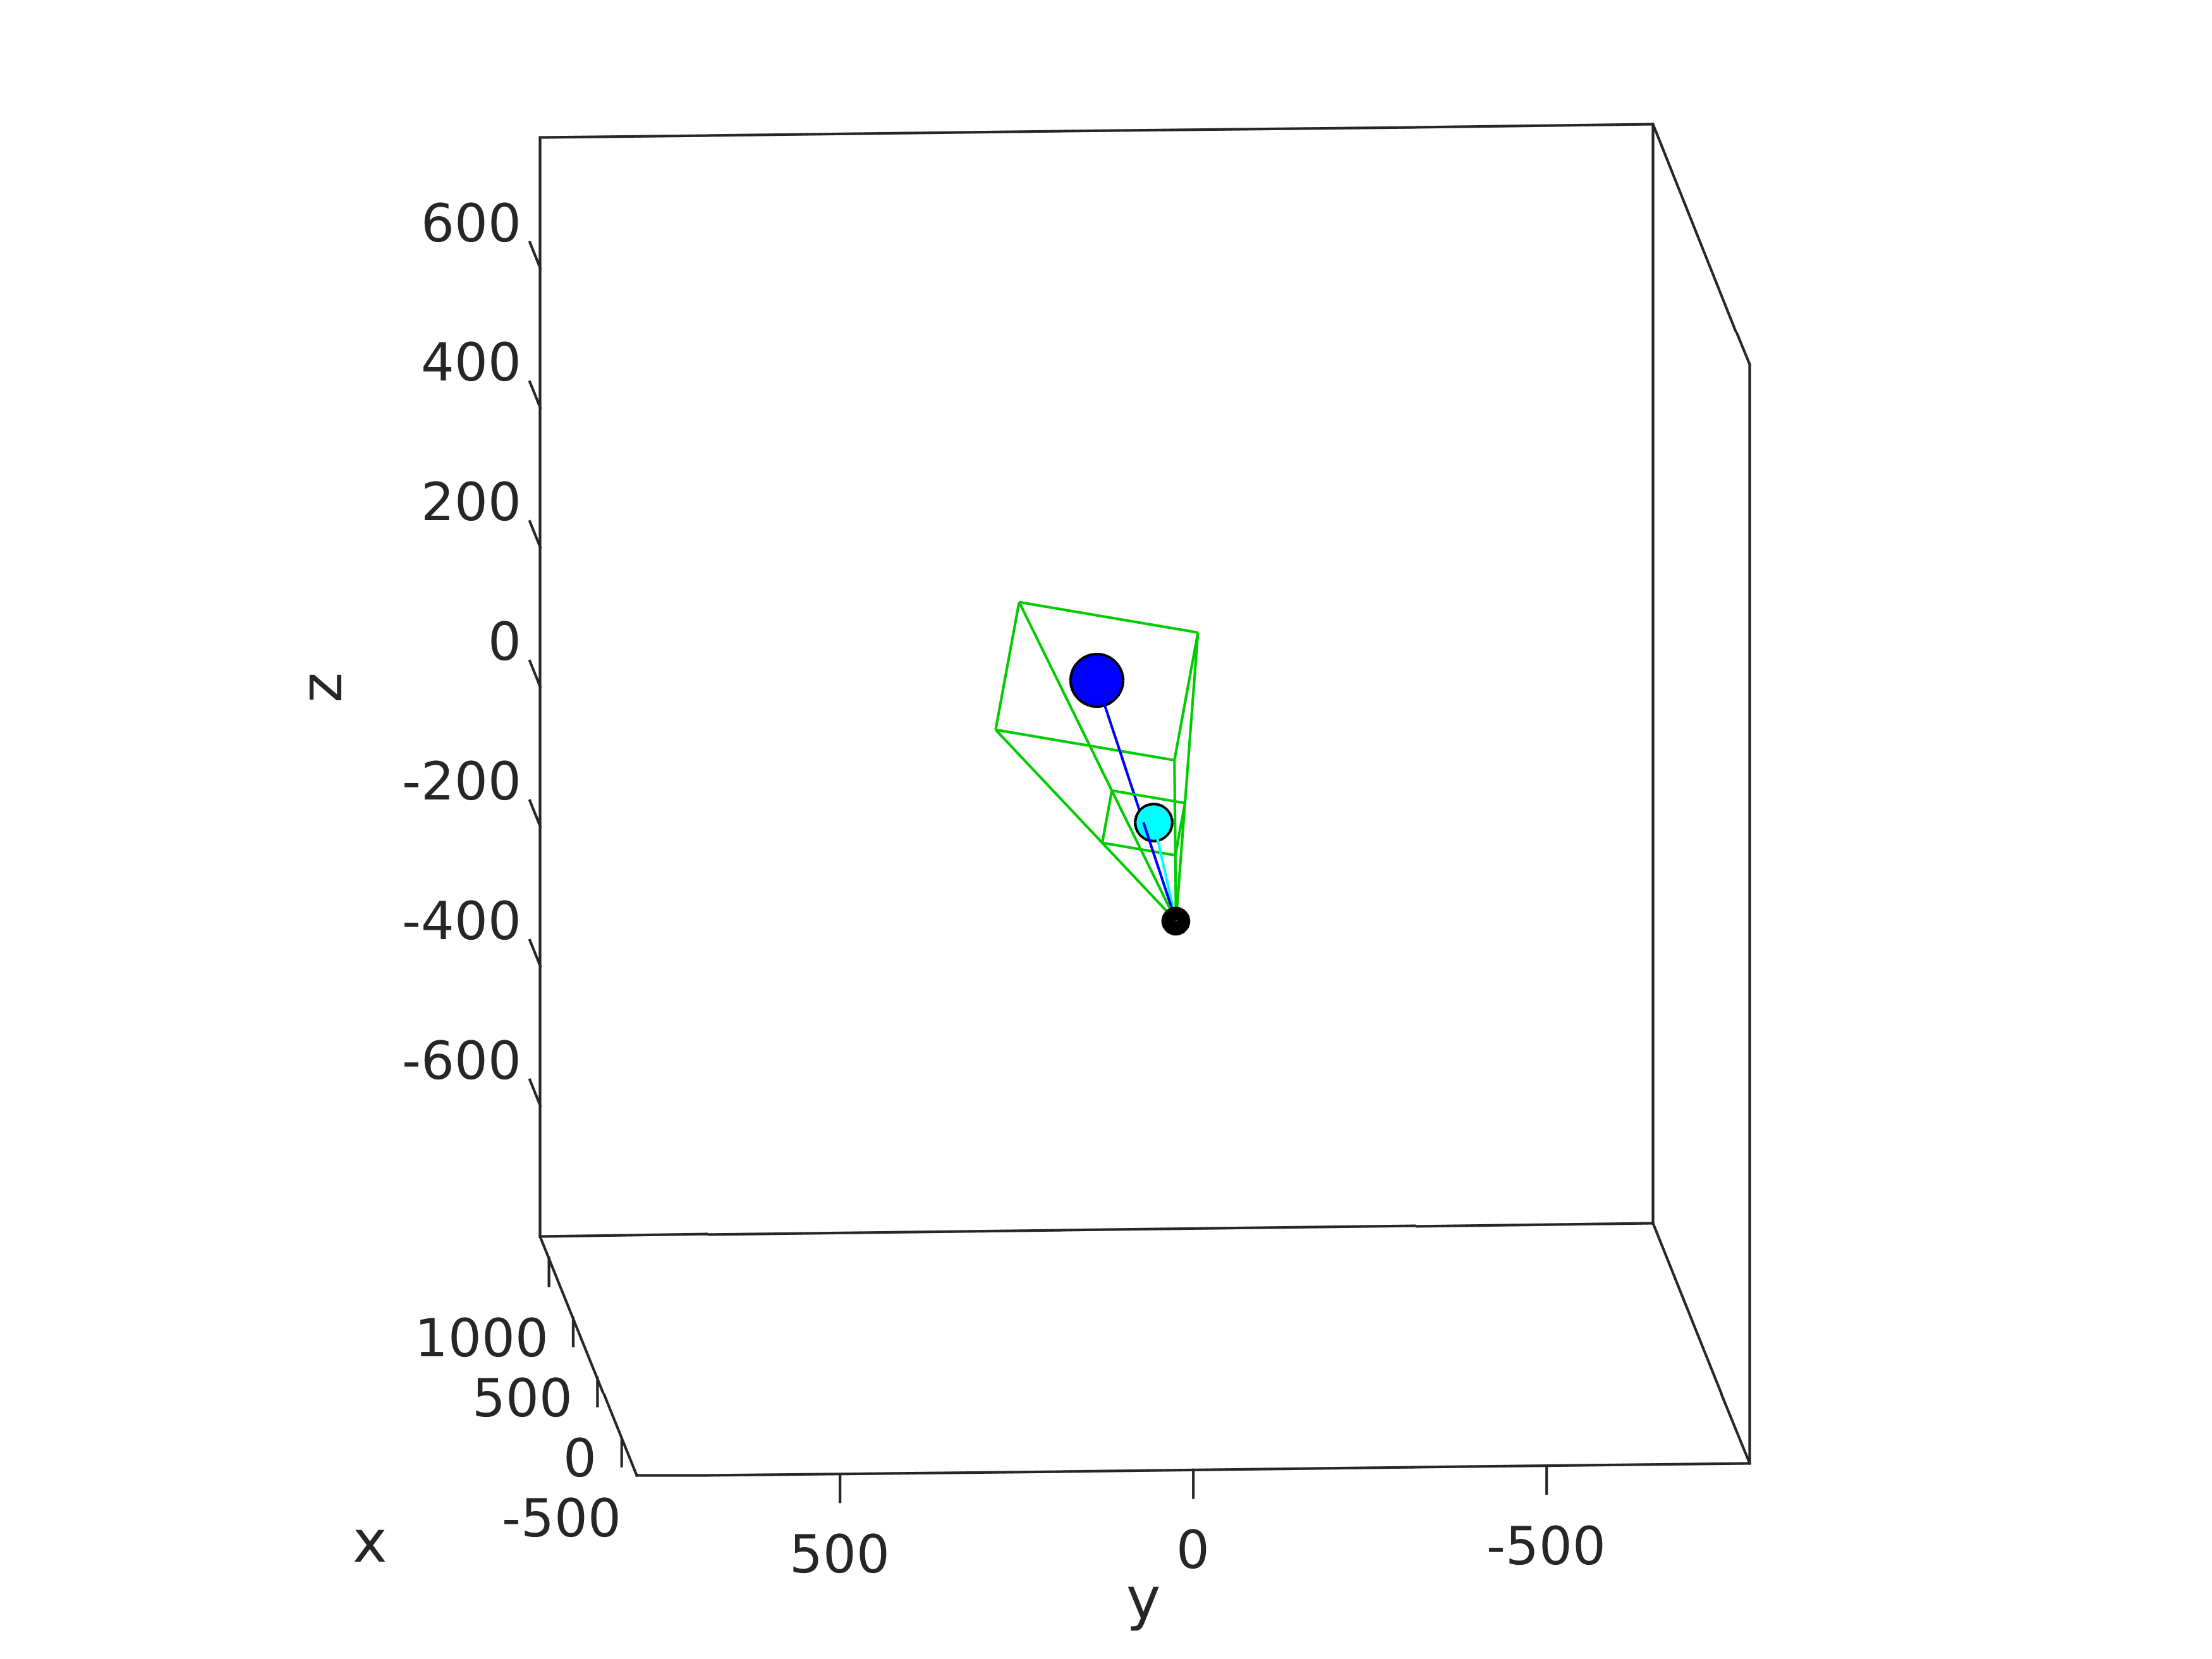
\includegraphics[width=0.49\linewidth]{rsc/cosmo-matlab2.png}
    \caption{View from HERA on the binary system of asteroids Didymos reconstructed on MATLAB. The black dot is the spacecraft HERA, the cyan dot is Didymoon and the blue dot is Didymain. The two images are taken at the same time as in \autoref{fig:9.1}.}
    \label{fig:9.2}
\end{figure*}

In order to get a more visual grasp on HERA's vision on Didymoon, it is possible to make us of the NASA/NAIF Spice database, coupled with Cosmographia. 

Spice is an observation geometry information system designed by NASA's Navigation and Ancillary Information Facility (NAIF) to assist scientists in planning and interpreting scientific observations from space-based instruments aboard planetary spacecraft. 

Cosmographia is an interactive tool used to produce 3D visualizations of planet, spacecraft and other objects in the solar system, while taking into account trajectories positions and orientations. 

By combining known positions of Didymoon, Didymain, expected positions of HERA and the characteristics of the on-board AFC -- Asteroid Framing Camera, the objective is to recreate a visual representation of the visibility HERA will have on Didymoon during the various mission phases. 

It relies on the FOV condition API set of functions --cspice\_fovray -- provided in the NAIF Spice toolkit which verifies if a ray is withing the boundaries of a specified instrument. By using this API, it is theoretically capable to determine which parts of Didymoon are visible at any moment in time. 

A script has been written to reproduce the view of \autoref{fig:9.1} in MATLAB for easier studies and it gives \autoref{fig:9.2}. The script detects wheter Didymoon is outside the field of view of the framing camera as shown in \autoref{fig:9.3}.

\begin{center}
    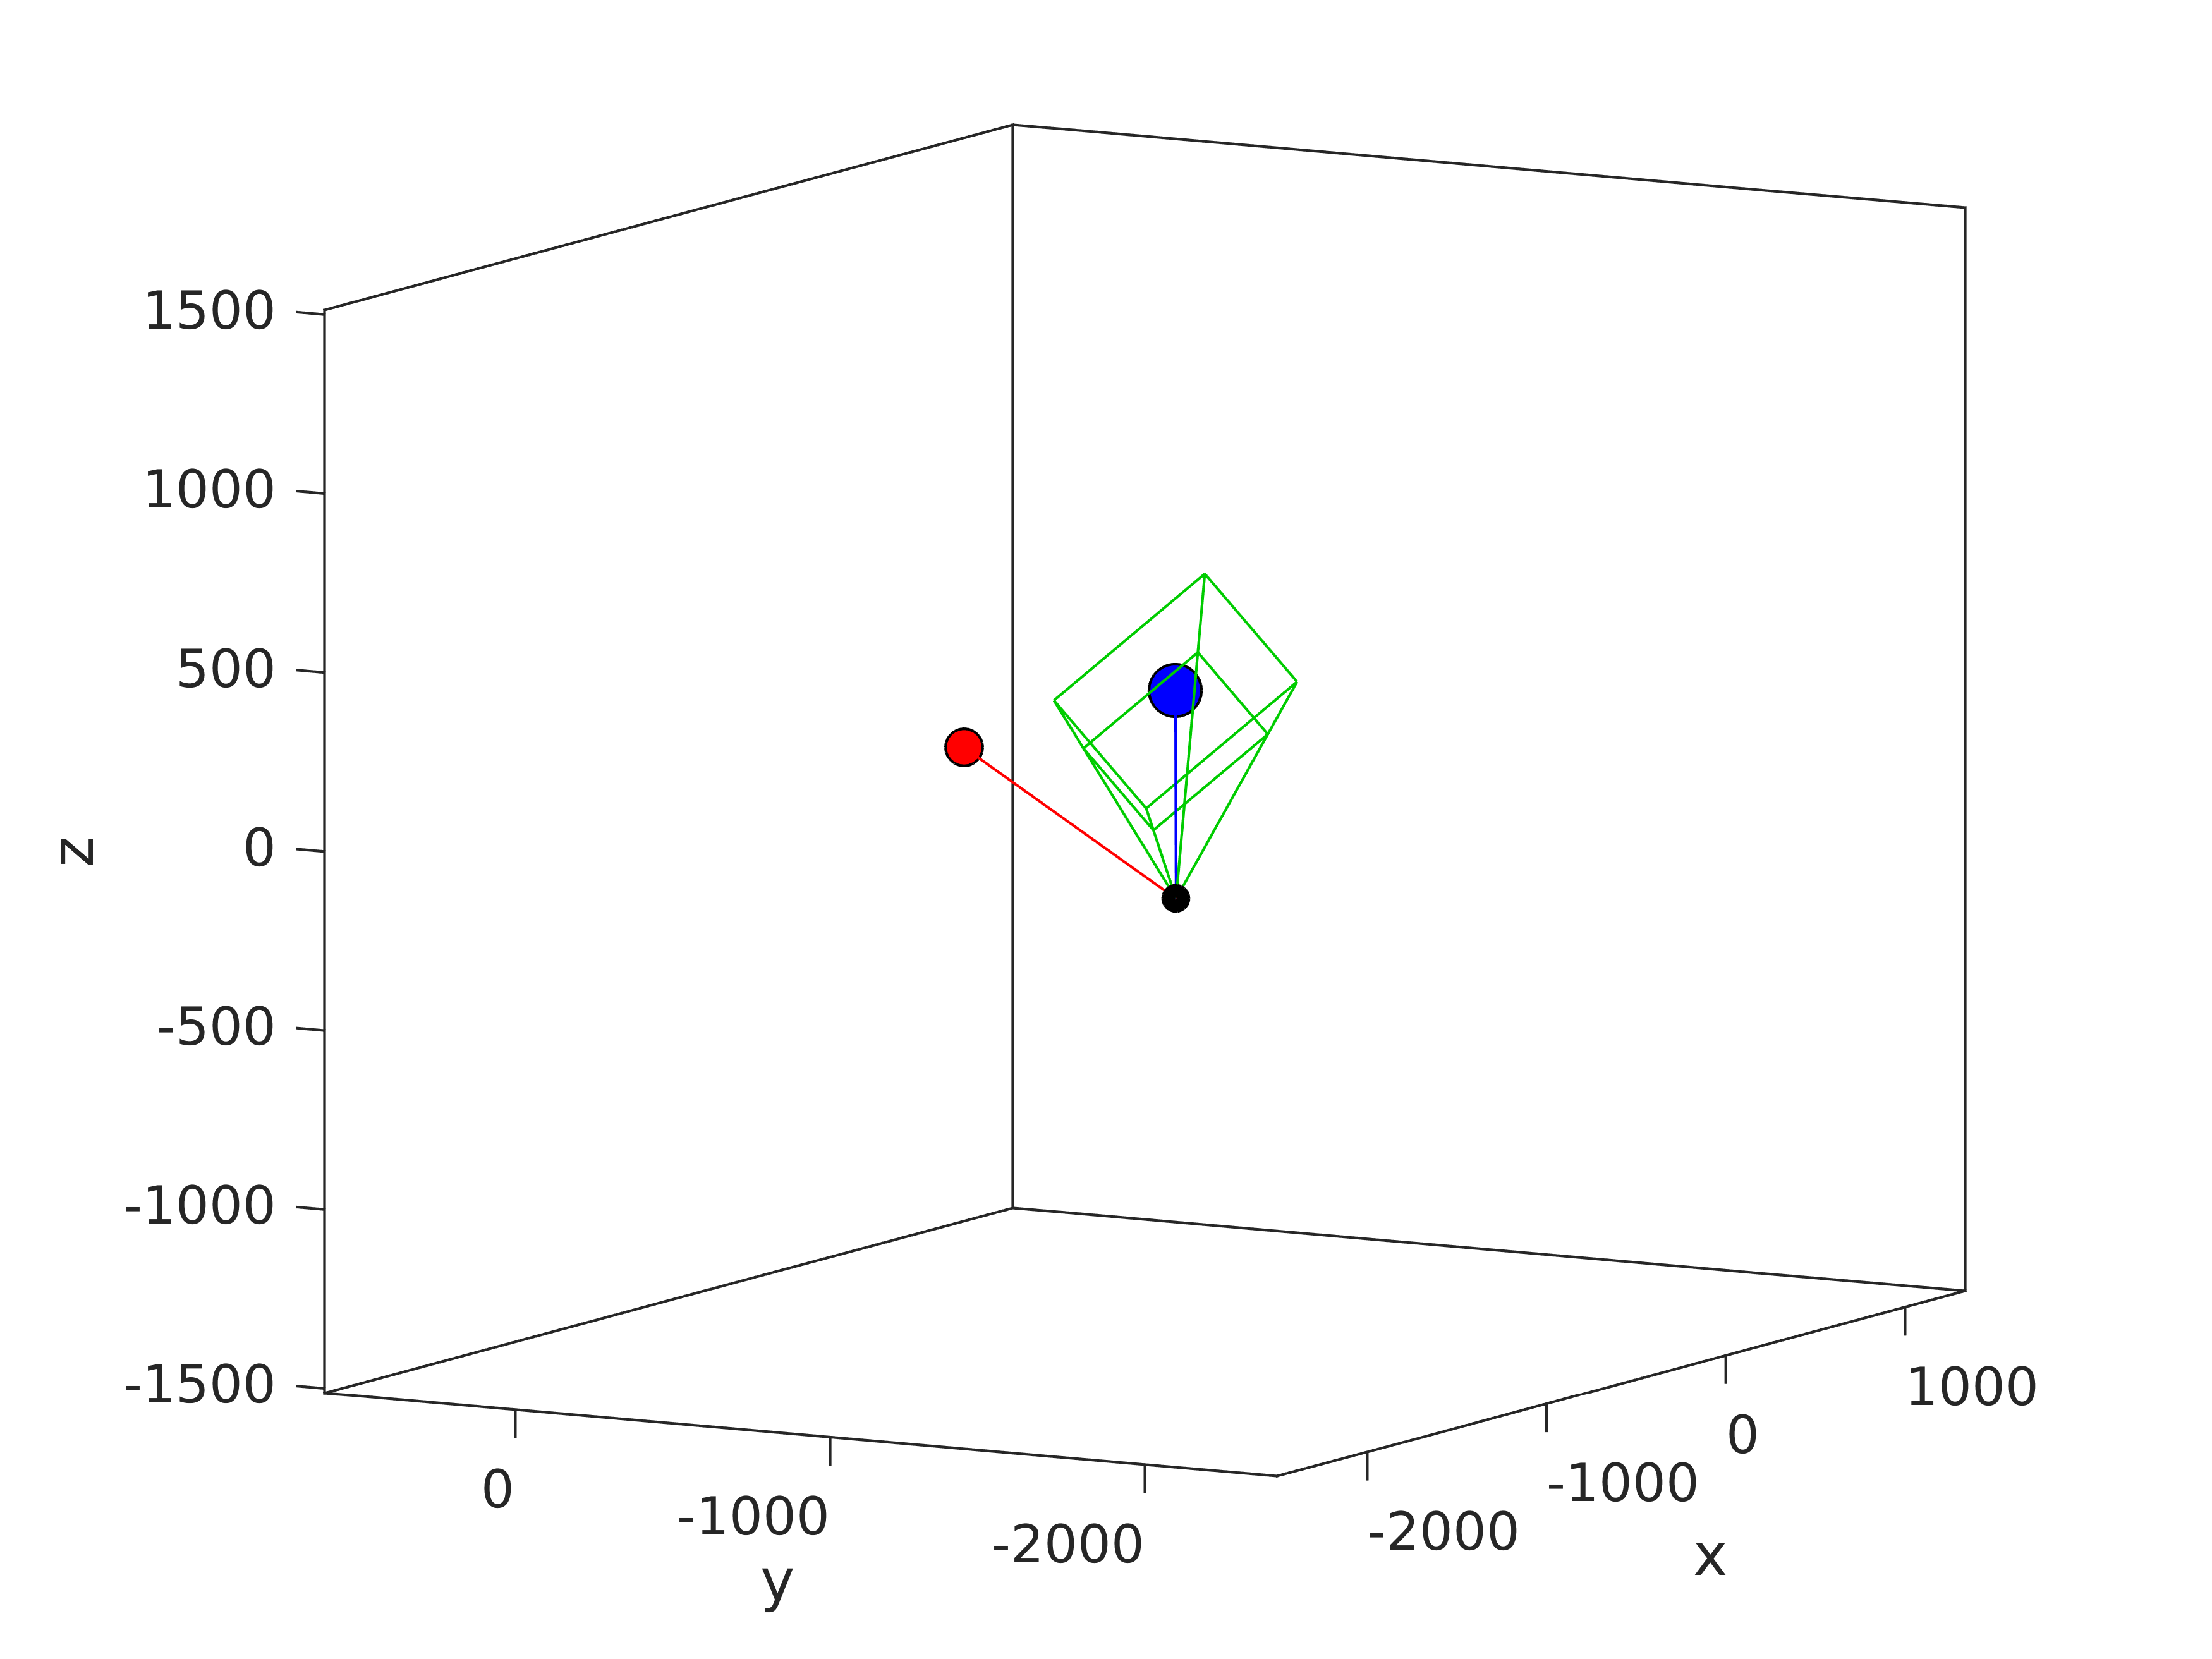
\includegraphics[width=0.6\linewidth]{rsc/cosmo-matlab3.png}
    \captionof{figure}{Example of the detection of the absence of Didymoon in the field of view of the framing camera. Didymoon appears in red as it is outside the field of view.}
    \label{fig:9.3}
\end{center}

\autoref{fig:9.2} and \autoref{fig:9.3} show the results wheter Didymoon is visible by the framing camera on board to HERA. Another aim of this document is to determine is the percentage of visible surface. \autoref{fig:9.4} shows the results.

\begin{figure*}[t]
    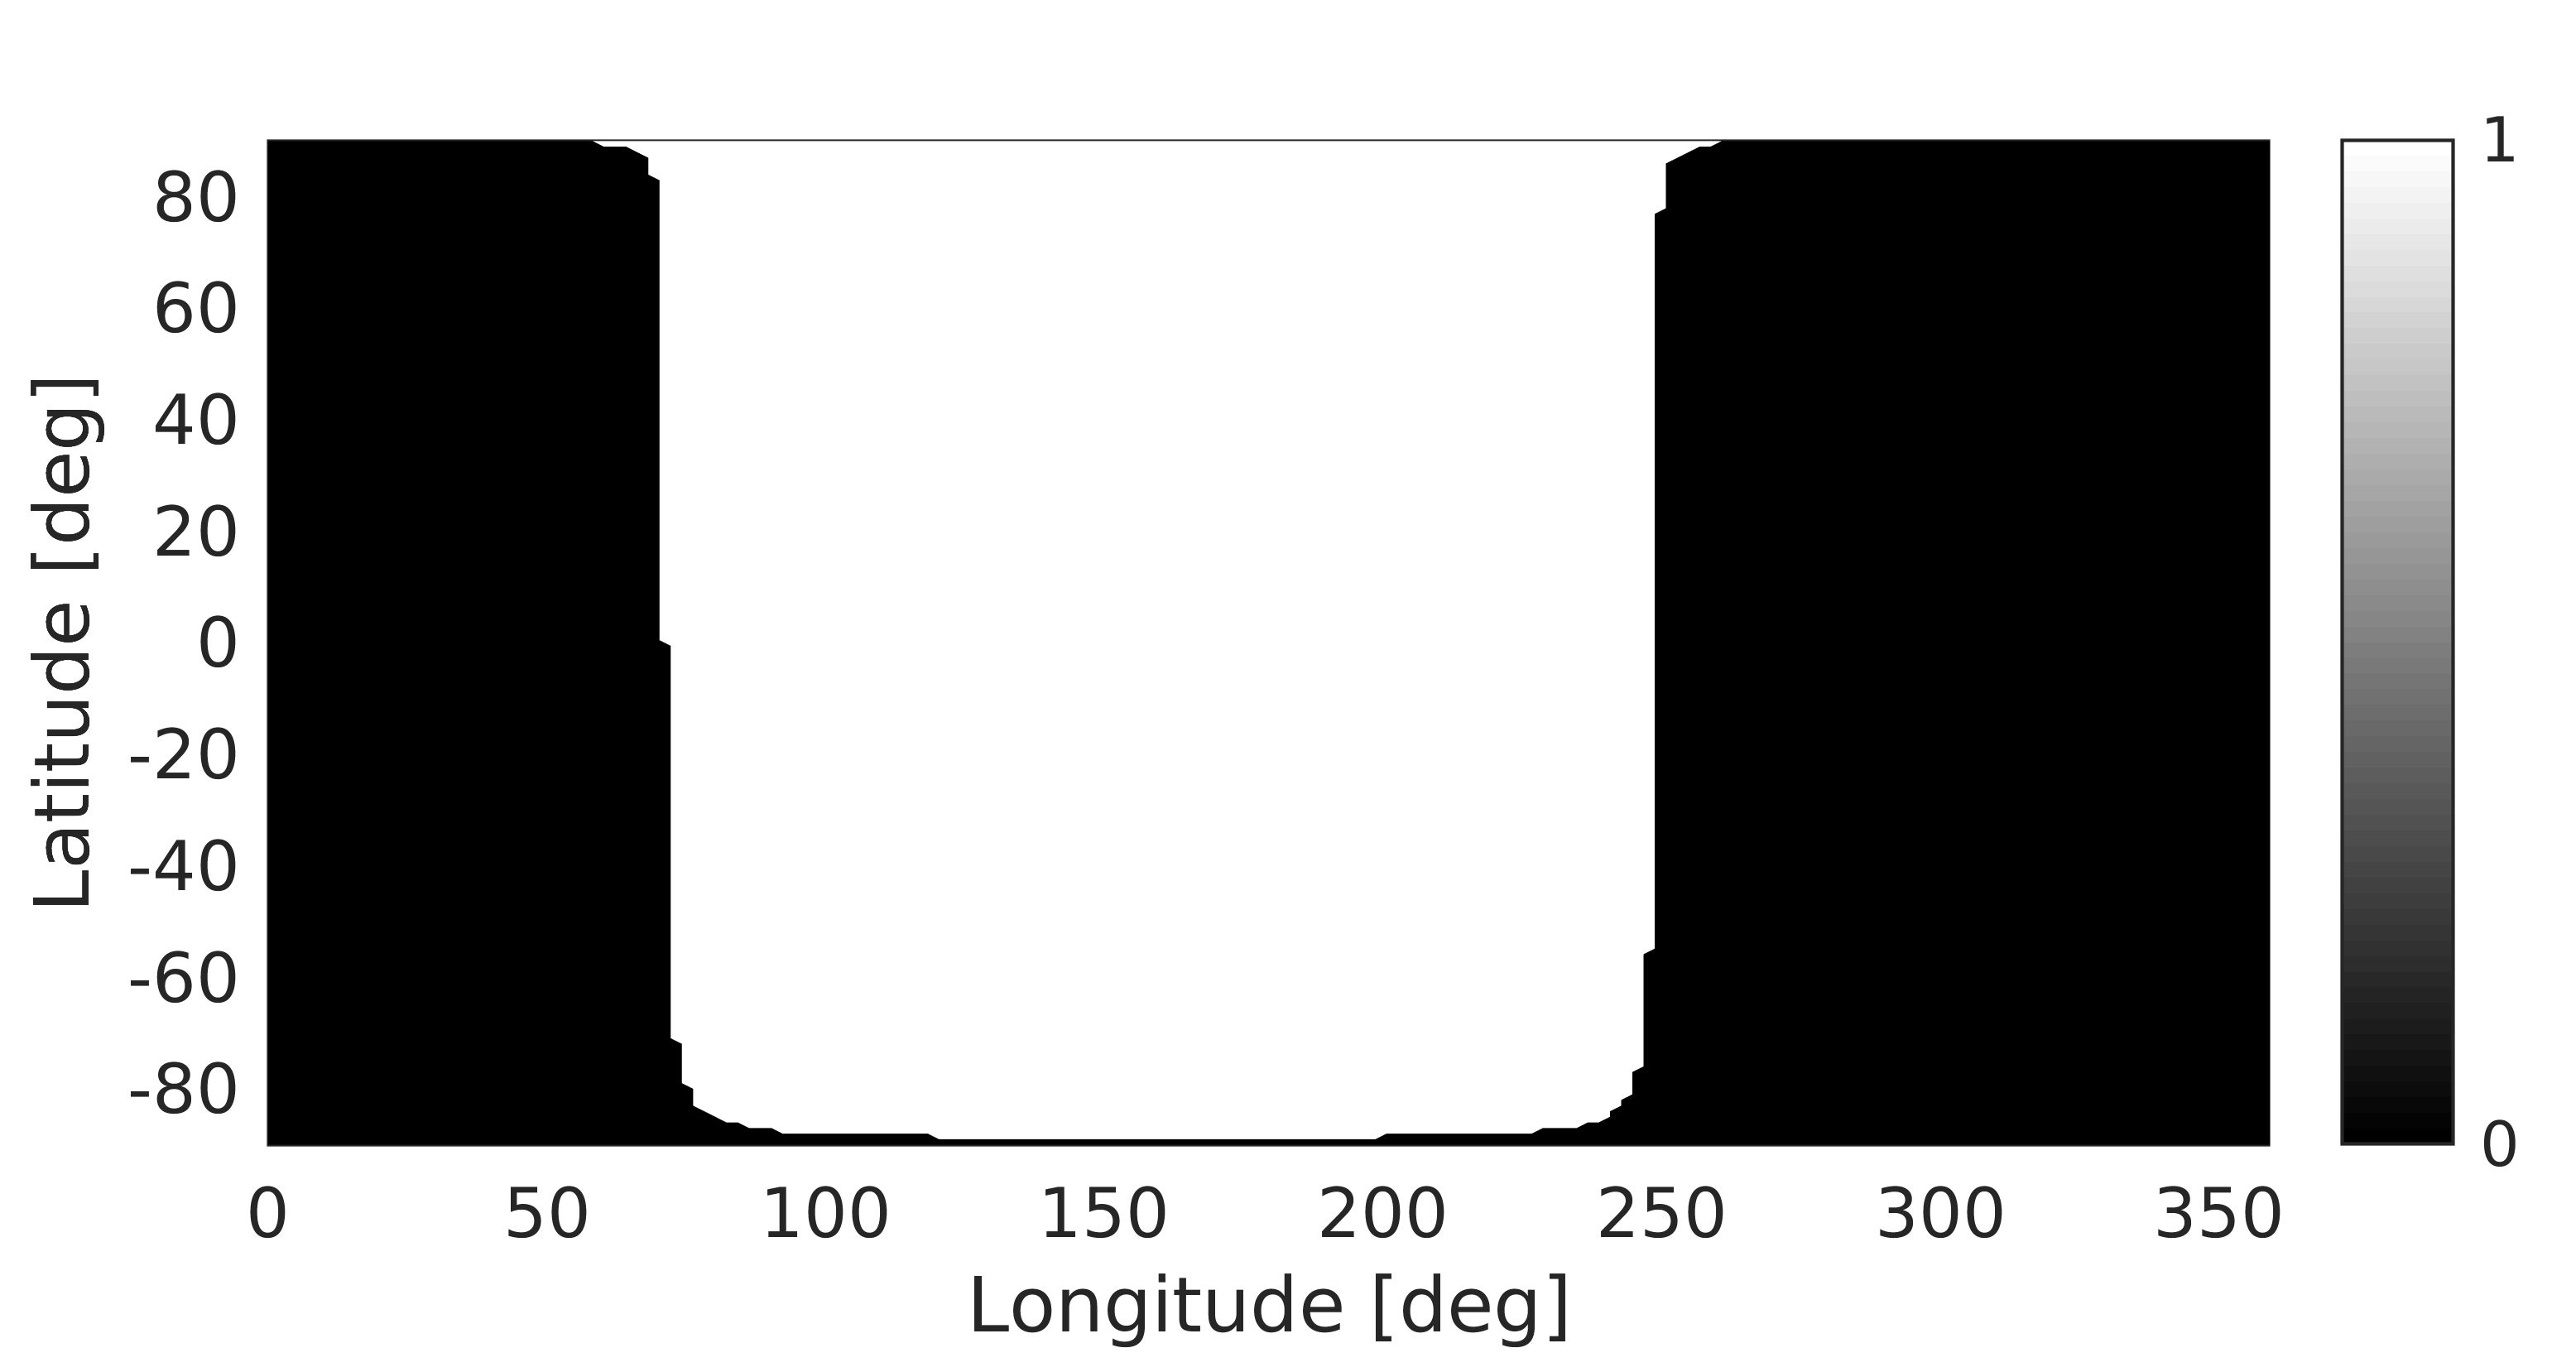
\includegraphics[width=0.49\linewidth]{rsc/areacov1.png}
    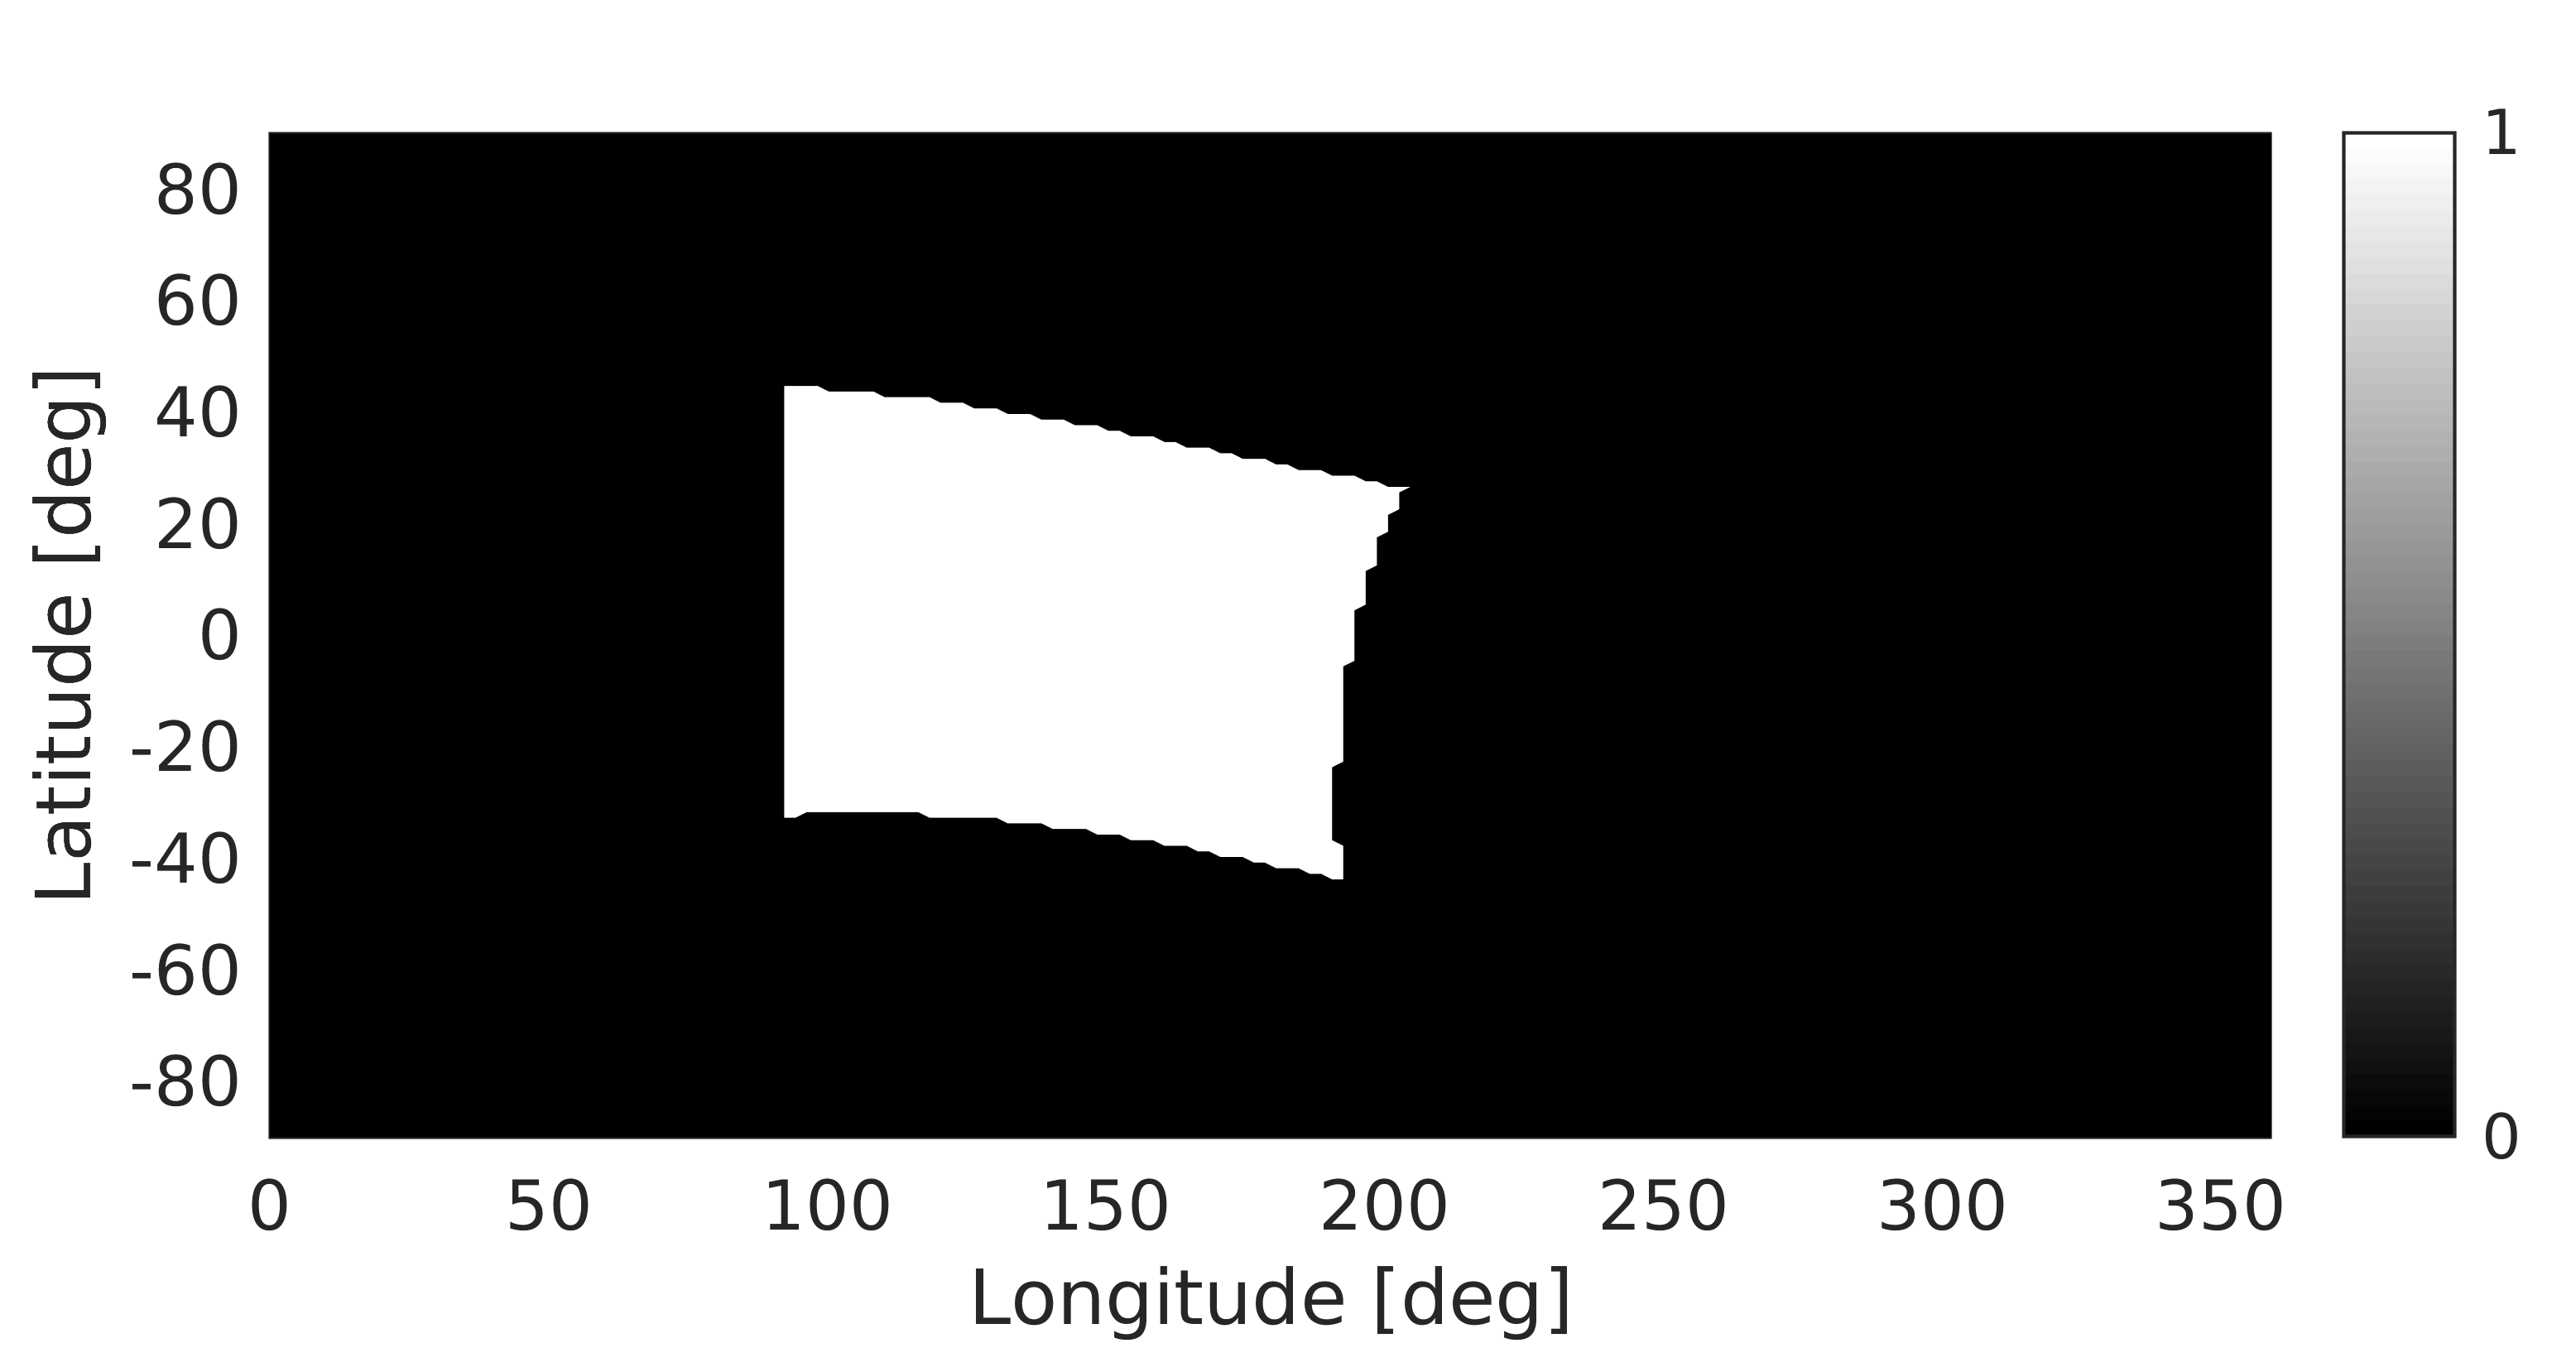
\includegraphics[width=0.49\linewidth]{rsc/areacov2.png}
    \caption{Percentage of visible surface of Didymoon. The two images are taken at the same time as in \autoref{fig:9.1}. The region in white represents the visible surface.}
    \label{fig:9.4}
\end{figure*}

There seems to be a small difference from the reality in the second image of \autoref{fig:9.4}. After studying the different possibilities to explain the cause, we have observed this weird-looking occurs only during the closest flyby of 1 \si{AU}. The visible surface is theoritically supposed to be the cross section of a sphere -- this case actually happens at infinite distance from the observer to the sphere. The visible surface tends to reach half of the sphere. The closer the observer is to the object, the smaller the visible area must be. Further works will consist into studying this phenomenon.
